\documentclass[UTF8]{ctexart}
% \documentclass{article}
\usepackage{geometry, CJKutf8}
\geometry{margin=1.5cm, vmargin={0pt,1cm}}
\setlength{\topmargin}{-1cm}
\setlength{\paperheight}{29.7cm}
\setlength{\textheight}{25.3cm}

% useful packages.
\usepackage{amsfonts}
\usepackage{amsmath}
\usepackage{amssymb}
\usepackage{amsthm}
\usepackage{enumerate}
\usepackage{graphicx}
\usepackage{multicol}
\usepackage{fancyhdr}
\usepackage{layout}
\usepackage{listings}
\usepackage{float, caption}
\usepackage{graphicx}
\usepackage{subfigure}


\lstset{
    basicstyle=\ttfamily, basewidth=0.5em
}

% some common command
\newcommand{\dif}{\mathrm{d}}
\newcommand{\avg}[1]{\left\langle #1 \right\rangle}
\newcommand{\difFrac}[2]{\frac{\dif #1}{\dif #2}}
\newcommand{\pdfFrac}[2]{\frac{\partial #1}{\partial #2}}
\newcommand{\OFL}{\mathrm{OFL}}
\newcommand{\UFL}{\mathrm{UFL}}
\newcommand{\fl}{\mathrm{fl}}
\newcommand{\op}{\odot}
\newcommand{\Eabs}{E_{\mathrm{abs}}}
\newcommand{\Erel}{E_{\mathrm{rel}}}

\begin{document}

\pagestyle{fancy}
\fancyhead{}
\lhead{马浩天, 3240102534}
\chead{数据结构与算法第五次作业}
\rhead{Oct.16th, 2024}

\section{remove 函数的改进}
原有的 remove 函数在需要删除当前节点,且左右子树都存在的情况下采取如下操作:在右子树中寻找最小的元素,赋给当前节点,然后递归地删除右子树中最小的节点。事实上,这个过程只会发生一次,因此在树高合理的情况下,仅仅考虑树的结构的话,时间复杂度可以接受。唯一的问题在于\textbf{赋值}操作时间复杂度的不可控性。

为了改进这个问题,我在不改变原有删除思路的条件下,优化了赋值操作。首先,我写了 detachMin 方法,作用是:“查找子树中最小元素,删除所在节点,并返回节点的指针。”随后,在 remove 函数中我先调用 detachMin 方法寻找并删除右子树中最小节点,将返回的节点的左子树和右子树分别指向欲删除节点的左右子树,这样就可以直接将当前指针指向返回的节点。最后删除了返回的指针,这样就避免了 element 的复制,也不会产生内存泄漏。

(另一个做法是采用 std::remove 来进行移动赋值。我不知道哪个更好。)

\section{测试程序}
在原有测试程序的基础上,我修改了 printTree 的实现,使得它还将节点的深度输出,从而我们可以通过 printTree 重建整颗树出来。然后,单独对于 remove 做了一个测试,测试的树如下。
按照预期,程序输出了应有的树结构,并且在 valgrind 的测试下,没有出现内存泄漏。

\begin{figure}[htbp]
    \centering
    \subfigure[tree1]{
    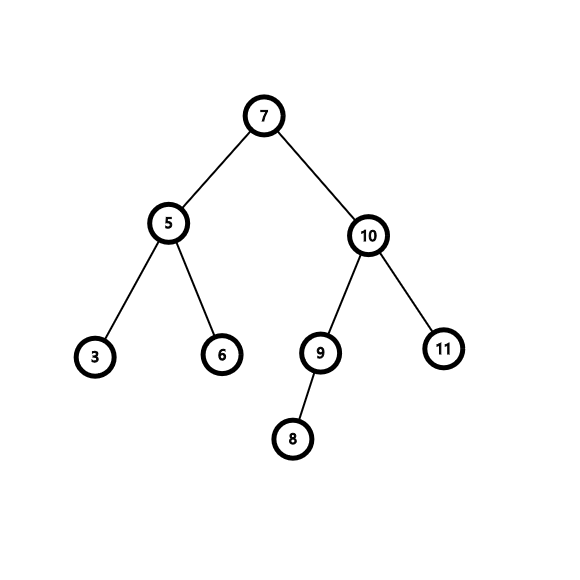
\includegraphics[scale=0.25]{tree1.png} \label{1}
    }
    \quad
    \subfigure[tree2]{
    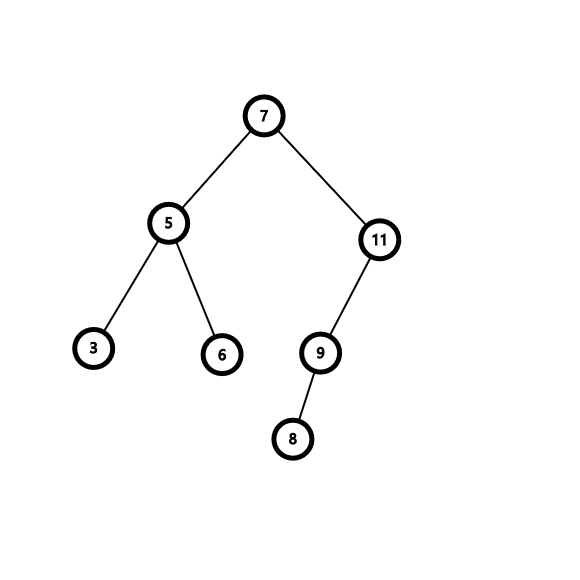
\includegraphics[scale=0.25]{tree2.png} \label{2} 
    }
    \quad
    \subfigure[tree3]{
    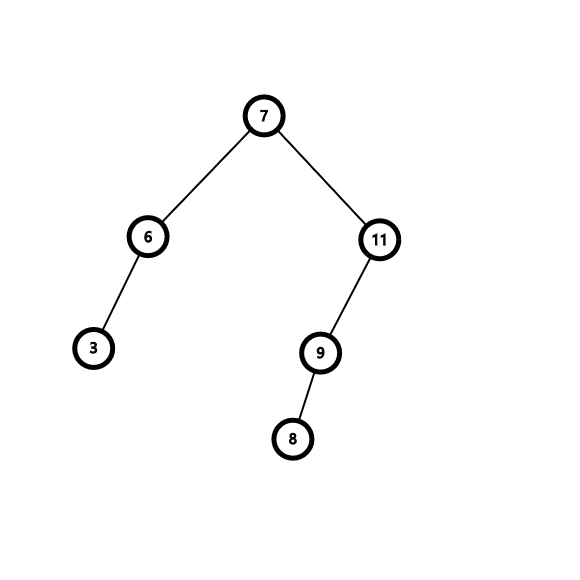
\includegraphics[scale=0.25]{tree3.png}\label{3}
    }
    \quad
    \subfigure[tree4]{
    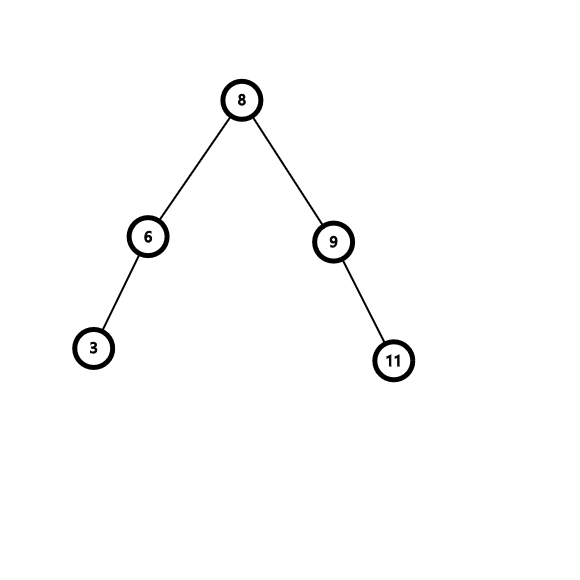
\includegraphics[scale=0.25]{tree4.png}\label{4}
    }
    \caption{删除10,6,7前后树的形态}
\end{figure}

\end{document}

%%% Local Variables: 
%%% mode: latex
%%% TeX-master: t
%%% End: 
